\section{Ursprung}

Wie im Artikel zu \ac{DevOps} auf den Seiten 10 und folgende des Magazins Objektspektrum 06/20 \cite{spektrum1} kurz angesprochen, beruht die Idee von \ac{DevOps} ursprünglich nicht auf Prinzipien aus der IT, sondern Prozessideen aus der industriellen Anfertigung, vor allem aus den Produktionshallen von Toyota. Von dort werden auch die Ansätze des Lean Managements und Kanban genutzt, die beide die Prozesskette als sehr wichtig betrachten und als Grundidee haben, dass sich die einzelnen Teilprozesse untereinander verständigen und abstimmen, um insgesamt den Prozess effizienter und stabiler zu betreiben. Insgesamt ging es bei Toyota damals im Bezug auf die effizientere Gestaltung der Prozesskette darum, alles darauf auszulegen, dass die Zeitspanne zwischen der Erteilung eines Auftrags bis zu dem Zeitpunkt, an dem das Geld fließt, so stark verkürzt wird wie möglich. \cite{halstenberg:2020} Das ist unter anderem durch weglassen unnötigen Aufwands (im japanischen \glqq Muda\grqq\ genannt) und die effizientere Gestaltung einzelner Teilprozesse durch die Nutzung der Ideen von Kanban und Lean zu erreichen. Kanban beschreibt grundsätzlich das Konzept, dass jeder Teilprozess eigenständig seine Produktion verwaltet, d. h. jede Abteilung fordert selbst an, wie viele Ressourcen benötigt werden und auf der anderen Seite produziert jede Abteilung nur genau so viel, wie die folgende Abteilung anfordert. Dadurch wird eine zentralisierte Ressourcenverteilung in den Hintergrund gestellt, und jede Abteilung ist selbst verantwortlich, das sie grundsätzlich am besten weiß, was gerade wie viel benötigt wird \cite{ohno:1988}. Die Ideen des Lean Managements werden in den folgenden Abschnitten angesprochen und vor allem in \autoref{sec:calms} genauer beschrieben.

Das Wort \ac{DevOps} ist das erste Mal während einer Konferenz im Jahr 2009 als Hashtag auf Twitter gestartet. Einige Monate später gab es eine erste Konferenz namens \glqq DevOpsDays\grqq\ in Gent, mit deren Start sich das Konzept von \ac{DevOps} rasant verbreitete \cite{halstenberg:2020}.

\section{Leitsatz}

Auch wenn mit der Philosophie des \ac{DevOps} einige Tools und Methoden gegeben werden, um die Überwindung der Wall of Confusion zu erreichen, so ist \ac{DevOps} doch viel mehr auch eine strukturelle Denkweise, die viel Arbeit braucht, um sie in den Köpfen der Nutzenden zu verankern. Es ist wichtig, sich als Nutzer von \ac{DevOps} immer wieder darauf zurück zu besinnen, dass \ac{DevOps} ein kontinuierlicher Prozess ist, der immer und immer wieder neue und alte Arbeit fordert.

Wie zuvor schon erwähnt ist es wichtig, von der Silodenke wegzukommen und sich und seine Abteilung nicht als eigenen Block zu sehen, der seine Arbeit macht und dann fertig ist, sondern dass man selbst weiß, wo man im Gesamtprozess einzuordnen  ist und wie die eigene Arbeit mit der Arbeit anderer Teilprozesse bzw. Abteilungen zusammenhängt. Unter anderem ist es dafür wichtig zu wissen, was und wie die anderen Teilprozesse arbeiten und was dort als Input bzw. Output erwartet wird. Im Lean Management wird in diesem Zusammenhang von internen und externen Kunden gesprochen. Die externen Kunden sind die klassischen Kunden, die als Außenstehende des Betriebs die Entwicklung eines Produkts in Auftrag geben. Das diese Art Kunde für den Prozess von großem Wert ist, steht außer Frage, da hiermit der zahlende Kunde gemeint ist. Der interne Kunde stellt das weitaus interessanteren Konzept dar, da hiermit alle Parteien gemeint sind, die irgendwie von einem Teilprodukt abhängig sind. Somit sind für einen Teilprozess alle anderen Teilprozesse, die letztendlich das Produkt der Arbeit aus dem Teilprozess erhalten, interne Kunden für diesen Teilprozess und müssen mit Kommunikation in die Arbeit und Gestaltung des Produkts mit eingebunden werden. Ein Team steht somit immer im Kontakt mit Teams, die ihr Produkt weiter verwerten sowie mit Teams, deren Produkte vom eigenen Team weiter verwertet werden. Das ist somit schon ein Konzept, um die Wall of Confusion, wie sie in \autoref{fig:wall} gezeigt wurde, einzureißen. Auch wenn zwei Abteilungen wie Dev und Ops scheinbar völlig entgegengesetzte Ziele erreichen wollen, so wollen alle, dass der Prozess erfolgreich beendet wird und das Produkt an den externen Kunden geliefert wird. Mit der Idee der internen Kunden können dann auch die scheinbar gegensätzlichen Ziele miteinander vereinbart und die Arbeit effizienter gestaltet werden.

Hierfür werden Prinzipien aus der agilen Entwicklung genutzt, unter anderem ein System von Feedforward und Feedback in kurzen Zyklen zwischen den beiden Abteilungen Dev und Ops, wie es in \autoref{fig:schleife} grob dargestellt ist.

\begin{figure}[h]
\centering
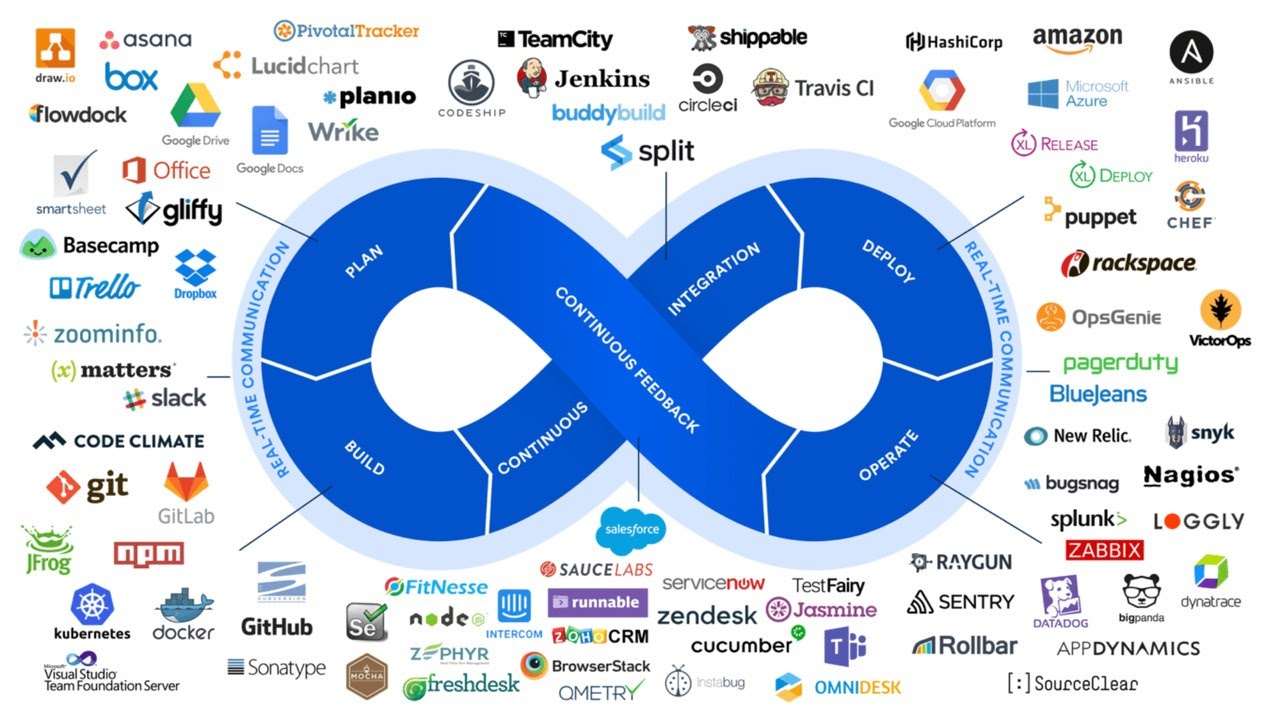
\includegraphics[width=\textwidth]{Graphics/devops}
\caption{\ac{DevOps} \cite{uplink:2021}}
\label{fig:schleife}
\end{figure}

Zu den Aufgaben des Developments auf der linke Seite in \autoref{fig:schleife} gehört das Planen (Architektur, neue Features usw.) und Bauen (Implementieren, Compilieren) der Software, wonach dann im Zusammenspiel mit den Operations eine \glqq continuous Integration\grqq\ stattfindet, also die Übergabe des Produktes von Dev zu Ops. Die Aufgaben der Operations beinhalten \glqq Deploy\grqq , also das Einsetzen bzw. Aufstellen der Software im Hardwarebereich sowie \glqq operate\grqq , womit das Benutzen der Software im gewollten Bereich gemeint ist. Als letzten Schritt wird hier das \glqq continuous Feedback\grqq\ genannt, welches wieder im Zusammenspiel mit der Abteilung des Development stattfindet. Sobald das Feeback beim Development angekommen ist, beginnt der Zyklus wieder von vorne mit der Planung und dem Bauen auf Seiten des Developments. Dargestellt durch die hellblaue Linie, die in \autoref{fig:schleife} die Schleife komplett einschließt, ist die kontinuierliche Kommunikation in Echtzeit. Jeder einzelne dieser Teilschritte wird in Kommunikation mit der jeweils anderen Abteilung abgearbeitet, es werden ständig Informationen ausgetauscht und Feedback eingeholt.

Die Tools, die um die Schleife herum in \autoref{fig:schleife} zu sehen sind, sind Beispiele für Programme, Methoden und Werkzeuge, die in den jeweiligen Schritten des \ac{DevOps}-Prozesses helfen können.

Ein wichtiger Punkt im Zuge des \ac{DevOps} ist auch die Etablierung von Fehlerkulturen, also das Akzeptieren von und Lernen aus Fehlern im Gegensatz zur Schuldzuweisung und den Versuchen, Verantwortung anderen anzuhängen. Mehr dazu jedoch in \autoref{chap:fehler}.

\section{CALMS}\label{sec:calms}

Das Akronym \glqq CALMS\grqq , welches auch als Säulen von \ac{DevOps} bezeichnet wird, steht für die Begriffe Culture, Automation, Lean Management, Measurement und Sharing. Diese Grundzüge von \ac{DevOps} müssen im Laufe der Integration von \ac{DevOps} in einem Betrieb immer wieder beachtet und neu verinnerlicht werden. Im Folgenden sollen diese Begriffe einzeln kurz erklärt werden, die Grundlage für diesen Abschnitt stammt aus dem Buch \glqq DevOps - Ein Überblick\grqq\ von Halstenberg \cite{halstenberg:2020}.

\subsubsection*{Culture}

Kultur ist einer der wichtigsten, wenn nicht sogar die wichtigste der Säulen von \ac{DevOps}. Wie zuvor schon erwähnt, ist \ac{DevOps} mehr als nur eine Sammlung von Methoden und Werkzeugen, es ist eine Philosophie zum strukturellen Umdenken der Kultur innerhalb eines Unternehmens. Es geht darum, dass sich Teilprozesse mehr als Teil eines ganzen, großen Prozesses sehen und nicht abgekapselt von anderen ihre Arbeit erledigen und ohne Feedback ihr Produkt weitergeben. Extrem wichtig für das Thema Unternehmenskultur ist das Vorleben der Kultur in den obersten und oberen Ebenen des Managements, sodass eine Vorbildfunktion entsteht, die der einfach Mitarbeiter vor Augen hat und der er folgen kann.

\subsubsection*{Automatisierung}

Für einen reibungslosen und effizienten Ablauf des Prozesses ist die Automatisierung von generischen und einfachen Aufgaben unabdingbar. Je mehr kleinste Teilprozesse automatisch ablaufen, desto eher kann sich die Arbeitskraft auf ihre Kernaufgaben konzentrieren und verschwendet nicht Stunden an Arbeitszeit z. B. u.a. daran, die Codebase zu versionieren. Auch automatische Unit-Tests nach jedem build sind Teil dieser Idee, da hier auf schnellste Art und Weise einfache, kleine Fehler früh erkannt werden können, die bei nicht-Beseitigung im späteren Lebenszyklus des Produktes zu schwerwiegenden Fehlern mutieren können.

\subsubsection*{Lean Management}

Das Lean Management, welches zuvor schon angesprochen wurde, beschreibt die Ideen des Toyota Production Systems und fand vor allem in den 1990er Jahren starke Verbreitung. Einige der Konzepte aus dem Lean Management wurden in vorhergehenden Abschnitten schon beschrieben, wie z. B. das Konzept des Kanbas (dezentrales Ressourcenmanagement) und die Idee von internen und externen Kunden. Wie man am Beispiel der internen/externen Kunden sieht, überschneidet sich die Säule des Lean Managements in Bereichen mit der Säule der Kultur sowie auch mit der Säule des Measurements, da auch das Konzept von kontinuierlicher Messung zur Verbesserung des Prozesses ein Teil des Lean Managements ist. Auch ein sehr wichtiger Punkt in den Prinzipien von Lean ist die Visualisierung von Arbeit, also die Idee, dass jeder zu jedem Zeitpunkt sieht, was wer gerade für Aufgaben erledigt. Diese Konzept ist auch heutzutage im puren Development weit verbreitet mit Werkzeugen wie Trello oder Issues bei der Nutzung von GitHub/GitLab. Dort können einzelne, kleine Aufgaben bestimmten Mitarbeitern genau zugeordnet werden und jeder kann einsehen, wer für das angegebene Problem zuständig ist. Im Zusammenhang hiermit steht auch die Idee, für jeden Mitarbeiter eine maximale Grenze zu geben, an wie vielen Aufgaben der Mitarbeiter gleichzeitig arbeiten darf. Das beugt Überlastung und Stress vor und führt meistens dazu, dass der Mitarbeiter sich besser und effizienter um seine aktiven Aufgaben kümmern kann. Auch zuvor schon kurz genannt ist die Idee des \glqq Muda\grqq , die darauf ausgelegt ist, jeden unnötigen Verbrauch von Ressourcen oder Zeit zu eliminieren und den Prozess so schlank wie möglich zu halten. Wie eingangs erwähnt, war das grundsätzliche Ziel der Prozessoptimierung bei Toyota die maximale Verkürzung des Zeitraums zwischen eingehen des Auftrags und Zahlung für das Endprodukt.

\subsubsection*{Measurement}

Wie im Abschnitt zu Lean erwähnt, überschneiden sich die Säulen von Lean und Measurement in einige Abschnitten. Die Säule des Measurements steht für die Messung von Resultaten im Prozess anhand von Kennzahlen, z. B. wie lange es dauert, bis ein Fehler behoben wurde oder bis eine Anforderungsänderung implementiert ist. Anhand von solchen Kennzahlen können Fehler oder Bottlenecks innerhalb der Prozesskette erkannt und beseitigt werden, was den ganzen Prozess effizienter und stabiler macht.

\subsubsection*{Sharing}

Die Säule des Sharings beschreibt die Idee des Informationsflusses in jede Richtung, wie er zuvor schon ausgiebig erläutert wurde. Hier wird wieder grundsätzlich aufgezeigt, dass die Teams nicht in Silos denken und sich einer eigenen Gruppe angehörig fühlen sollen, sondern in Zusammenarbeit und Kommunikation mit anderen Teams stehen sollen. Wichtig hierfür ist eine zuvor schon angesprochene Fehlerkultur (mehr dazu in \autoref{chap:fehler}), in der Schuldzuweisungen keinen Platz haben und Fehler eher als Lernprozess gesehen werden.

\section{Guiding Tools}

Da \ac{DevOps} keine Sache ist, die einmal in das Unternehmen eingebunden wird und ab dann perfekt funktioniert, müssen einige Dinge beachtet und kontinuierlich verbessert werden. In dem Artikel \glqq Law \& Order für DevOps\grqq\ auf den Seiten 28 und folgende des Magazins OBJEKTspektrum 06/20 \cite{spektrum2} werden einige Guiding Tools genannt, die einen Rahmen für das erfolgreiche Einsetzen der \ac{DevOps}-Struktur ermöglichen. Ein paar der dort aufgezeigten Konzepte sollen im folgenden genannt und kurz erklärt werden.

\subsubsection*{Zero Tolerance}

Entstanden im New York der 60er Jahre geht das Konzept der \glqq Zero Tolerance\grqq\ davon aus, dass selbst kleinste Fehler und Makel dazu führen, dass die Hemmschwelle für Fehler und Makel der gleichen Art sinkt und mehr solcher Probleme entstehen, z. B. führt dann eine eingeschlagene Scheibe an einem Haus dazu, dass noch mehr Vandalismus an dem Haus geschieht bis es irgendwann komplett zerstört ist. Um dem Problem entgegenzuwirken wurden selbst kleinste Delikte hart bestraft und die Makel (z. B. die eingeschlagene Scheibe) sofort beseitigt. Bezogen auf \ac{DevOps} geht es darum, selbst kleinste Fehler und Bugs sofort auszumerzen und nicht mit der Denkweise zu arbeiten \glqq kleine Fehler sind nicht so schlimm\grqq , was dazu führen kann, dass viele kleine Fehler auftauchen. Zu der Einhaltung der Zero Tolerance gehören noch viele weitere, kleinere Prinzipien, der Hauptpunkt dabei ist jedoch Disziplin in der Durchführung. Auch die folgenden Werkzeuge können dabei helfen, das Konzept der Zero Tolerance über den ganzen Prozess beizubehalten.

\subsubsection*{Skill Pump}

Die Idee des \glqq Skill Pump\grqq\ gibt eine mögliche Lösung für das Problem, dass eine gewisse Aufgabe mit der aktuell für die Aufgabe gegebenen Grundlage nicht lösbar ist. Sollte ein solches Problem entstehen, so besagt Skill Pump, dass zum erfolgreichen Absolvieren dieser Aufgabe die Grundlage verbessert werden muss, also wird \glqq Skill\grqq\ in die Grundlage \glqq gepumpt\grqq . Wie die Grundlage verbessert wird bleibt offen, es können z. B. Wissensträger oder Entscheidungsbefugte sein, je nachdem welche Ressource in dem spezifischen Fall benötigt wird. Das Ganze kann auch in Form von speziellen, kurzfristigen Rahmen passieren, ein prominentes Beispiel dafür ist eine sogenannte \glqq Task-Force\grqq .

\subsubsection*{Shift Left}

Mit dem Begriff \glqq Shift Left\grqq\ ist das Konzept gemeint, Fehler so früh wie möglich (so weit links im Prozess wie möglich) zu erkennen und beheben, da ein Fehler, je länger er unentdeckt bleibt, immer größeren Schaden anrichten kann. Ganz offensichtlich ist dieses Konzept ein Tool zur Erreichung der Zero Tolerance. Ein Beispiel hierfür sind die schon erwähnten automatischen Unit-Tests, die z. B. bei jedem Commit einmal laufen und mit denen kleine Fehler schnell und einfach gefunden werden können. Ein Problem bei diesem Konzept ist, dass hierbei tendenziell die Teams mehr belastet werden, die weiter links im Prozess arbeiten, in unserem Fall also das Dev-Team. Sollte nun ein Modul unerwartet viele Probleme aufwerfen, so ist es die Aufgabe des Dev-Teams, die Fehler alle so schnell wie möglich zu beheben. Deswegen muss ein solches Konzept wie das des Shift-Left Hand in Hand mit anderen Werkzeugen gehen, die den Stress und die Arbeitslast bei den Mitarbeitern in den betroffenen Teams verteilen oder abbauen. Ein Beispiel für ein solches Werkzeug wäre das (auch schon erwähnte) Begrenzen der Anzahl der Aufgaben, an denen ein Mitarbeiter gleichzeitig arbeiten darf.

\subsubsection*{Overall Code Control}
 
Der Leitsatz des Prinzips der \glqq Overall Code Control\grqq\ ist \glqq Don't touch the code without a ticket!\grqq . Die Idee ist, dass für bekannte Probleme und Aufgaben immer Tickets erstellt werden und Dinge nur bearbeitet und Probleme nur gelöst werden, wenn ein solches Ticket dazu besteht. Das Ticket wird dann mit einem bestimmten Mitarbeiter verbunden, der sich um die darin enthaltene Aufgabe kümmern soll. Insgesamt verhindert dieses Prinzip ungeplante oder sogar versteckte Arbeit, die niemand nachverfolgen kann, was immer zu Problemen führen kann. Hierfür wird heutzutage oft eine Kombination einer Versionskontrolle und eines Tools zur Verteilung von Tickets verwendet, wie z. B. das weit verbreitete Tool Git mit dem Tool Jira. Nun wird jeder Commit, der über Git abgegeben wird, einem bestimmten Ticket zugeordnet und es ist klar, welche Aufgabe mit dieser Code-Änderung bearbeitet wird.

